\begin{abstract}
\section{selection}
In this chapter we will explain how our selection system works. We will show which classes are involved and how the methods are chained using UML-diagrams. 

\subsection{User interface}
First off, how does the selecting feature works. You can select a unit by clicking on it using the left mouse button. You can select multiple by holding the left mouse button and dragging, while dragging a rectangle is drawn. This rectangle represents the selecting area. When you release the left mouse button every unit in the selecting area, the red rectangle, will be selected. Selected units are recognizable by the red line surrounding them.

\subsection{Detecting events}
To handle an event, we first need to detect it. We have a window a SDL window that represent the world. We want to detect the mouse events that are used on this window. This is done using two while-loops. First we have a while-loop that runs as long as the game is running. In this while-loop we want to detect the events. So we have a while-loop that uses the SDL\_PollEvent method to poll for events. A code snippet of this while-loop can be found below.

\begin{figure}[!htb]
    \centering
    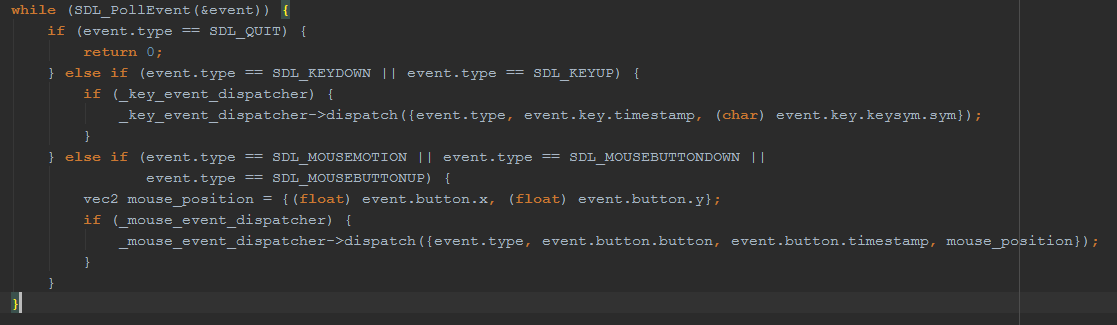
\includegraphics[scale=0.75]{images/PollingEvents.PNG}
    \caption{Detecting events in the world window.}\label{fig:fuzzy-distance}
\end{figure}
\newpage

We first determine what kind off event is executed using if-statements. When the event type is either a motion of the mouse, a button up or a button down we call the mouse event dispatcher and set the parameters of the executed event. This mouse event dispatcher calls the handler of the mouse events which is explained in the next sub chapter.


\subsection{Handling events}
First we made a handler that handles mouse input from a panel that represents the world in the user interface. This is the MouseHandler class, it derives from the SDL\_MouseEventSlot class which derives from the Slot class. SDL is a library that helps making a user interface in C++. The SDL library provides us with low level access to the mouse input on the panel. The header file of the MouseHandler can be seen below.

\begin{figure}[!htb]
    \centering
    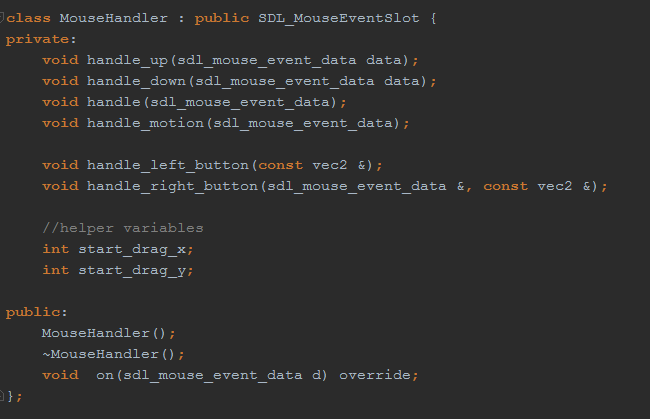
\includegraphics[scale=1.0]{images/MouseHandler.png}
    \caption{The MouseHandler class.}\label{fig:fuzzy-distance}
\end{figure}

\newpage
The class has a lot of private methods that handle the user input separately. It has one method that has been overridden from the base class, which is the on-method. The on-method is where user inputs comes in. In this method the input is separated into two groups and will be handled further by other methods. To make clear how this works an explanatory activity diagram can be found below to illustrate the process. Below the image we will globally explain what the methods do individually. 

\begin{figure}[!htb]
    \centering
    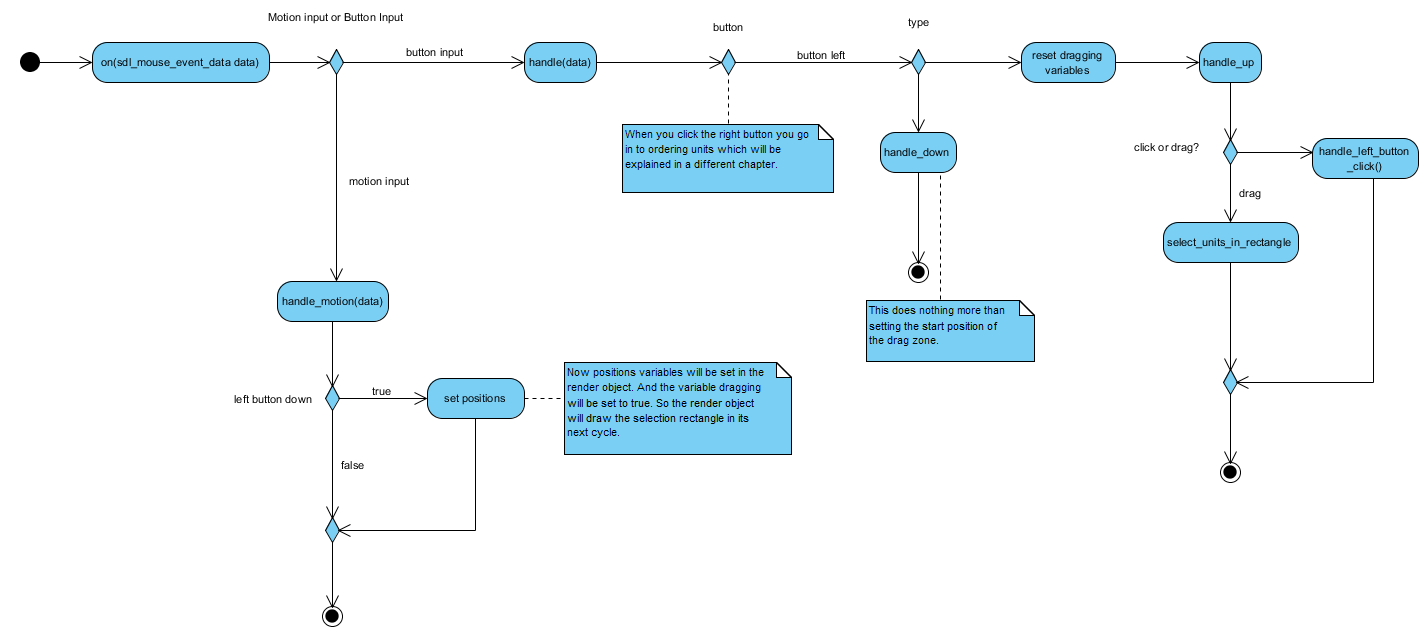
\includegraphics[scale=0.55]{images/ActivityDiagramMouseHandler.PNG}
    \caption{Handling user input activity diagram.}\label{fig:fuzzy-distance}
\end{figure}

If the text in the image is unreadable, we recommend taking a look at the PNG file in the images folder.

After the on-method has determined whether the incoming data is a motion event or button it will be handled further by other methods. We will start with a motion input.

Motion input is handled by the handle\_motion function. Motion is only important for us when the user is dragging. This means the user is holding the left mouse button down while moving the mouse. When the user is dragging we set the position the mouse has moved to and let the UI component know that the user is dragging by setting a variable dragging to true. The UI component has two methods called draw\_selection\_rectangle and render. Whenever the render method is called and the variable dragging is true it will call the draw\_selection\_rectangle with the positions set in the latest motion event handler.

Button input is handled a bit differently since we first need to determine what kind of event it is and from which button. If the event comes from the right button, it is an event that will control units. Since that has nothing to do with this topic we will leave it there and explain it in a different chapter. 

If however the event does come from the left button it is to select units. When the left button is pressed down we get the position of the cursor when it left button was pressed down. This will be the start position of the selection rectangle.   

Inevitably after a button down event from the left button a button up event will be fired from the button. This event means a few things. First off all the user has stopped dragging, cause we stated earlier that the user is dragging when is holding down the left button. So, we reset the dragging variable to false. Also we reset the positions to be ready for a next drag event. After resetting the variables, we call the handle\_up method. This determines whether the event was a drag or a click of the left mouse button. A click is when you press and release the mouse in the same position or at maximum 10 pixels away from the original position. We have implemented it this way so it is easier to click moving targets. The handle\_left\_button\_click is called and it selects the target on the clicking position, unless there is no target in range.

When you release the left mouse button more than 10 pixels away from the origin point you are dragging the mouse. The position of the release of the button and the position of the press will passed to the select\_units\_in\_rectangle method. The method first calculates the right, left, upper, bottom offset of the rectangle. After this all units inside will be selected. Below you can find a picture of a few units that are selected by the select\_units\_in\_rectangle function and you can also see the red rectangle that has been used to select them. 

\begin{figure}[!htb]
    \centering
    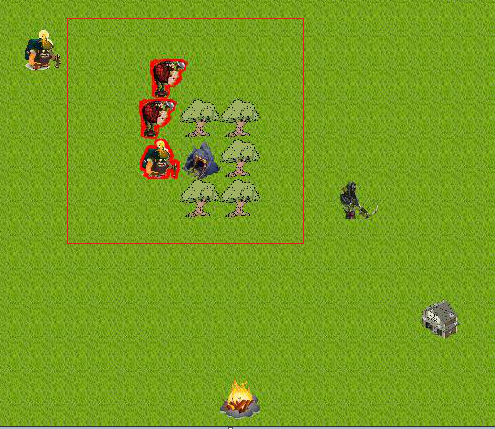
\includegraphics[scale=1.0]{images/SelectionRectangle.PNG}
    \caption{Selection by dragging the mouse.}\label{fig:fuzzy-distance}
\end{figure}



\end{abstract}
